	Sur ce projet j'ai été positionné en tant que développeur et ai donc travaillé directement avec l'équipe sur le développement du Fronting Digital. Ainsi, contrairement au projet mené chez Neuflize OBC, je n'ai pas réalisé différents travaux indépendants mais j'ai directement participé au développement de l'application. Cependant, nous avons adopté des méthodes agiles dont je vais parler plus en profondeur ci-dessous c'est pourquoi je ne peux pas détailler l'ensemble des tâches que j'ai effectuées, ces dernières étant nombreuses et toujours réalisées de la même façon au cours des différents sprints. Aussi, je vais plutôt d'abord expliciter le déroulement de ces sprints ainsi que la manière dont nous avons réalisé la conception des fonctionnalités ensuite de quoi je présenterai certaines tâches que j'ai effectuées en autonomie.

\subsection{Méthodes agiles}
	Comme nous l'avons dit plus haut, nous avons recours à un courant agile pour la réalisation de ce projet. Il s'agit d'une approche de gestion de projet qui vient s'opposer aux méthodes plus traditionnelles et séquentielles comme le \textit{cycle en V}. Ces pratiques traditionnelles sont le plus souvent dîtes de \textit{projet au forfait} où l'on établi en début de projet l'ensemble des relations commerciales et des obligations de chaque partie. L'intégralité du produit doit être spécifiée et plannifiée dans les détails ce qui aboutit à la création d'un cahier des charges très conséquent qui sera par la suite confié à l'équipe de développement. Après cela, les développeurs s'isolent sur une très grande période afin de déchiffrer ce cahier et de réaliser le produit. Le client doit avoir pensé à absolument tout, de la disposition des pages de son application à la couleur des boutons des formulaires. Les changements nécessites des avenants et sont réalisés souvent trop tard ce qui est contre-productif. De plus, tous les imprévus rencontrés lors de la phase de développement ont tendance à rendre la plannification de départ obsolète. \\
	
	Les méthodes agiles sont centrées sur la satisfaction du besoin client plutôt que sur la conformité d'un contrat et favorise un raisonnement "produit" plutôt qu'un raisonnement "projet". L'objectif est de ne mettre en place que des cycles courts nommés itérations et de découper le projet en plein de petits blocs. Le demandeur commence par exprimer ses exigences qu'il soumet aux développeurs en communicant directement avec eux, ce qui favorise l'entente et les relations et permet de gagner du temps. L'équipe choisit alors une partie des exigences ainsi qu'une courte période de temps pour effectuer les phases de spécification, conception, developpement et test, au terme de laquelle le produit est montré au client. Celui-ci peut alors émettre des feedbacks offrant de la \textbf{visibilité} qui seront pris en compte par l'équipe de développement. Cela favorise grandement l'entente et surtout la satisfaction du client c'est pourquoi il est crucial d'autoriser le changement. Ainsi, il est possible de s'\textbf{adapter} aux souhaits du demandeur, remplacer une fonctionnalité par une autre, modifier des styles, déplacer une page etc... et de réduire considérablement l'effet tunnel des approches classiques. En effet, il est possible d'éviter le surplus, les fonctionnalités qui ne seront finalement pas utilisées, de mettre en place les bonnes idées apparues pendant le projet et donc de véritablement enrichir le produit en mettant en avant la production de valeur pour l'utilisateur final (on parle de \textbf{business value}). Les \textbf{risques} repérés peuvent etre traités beaucoup plus tôt en travaillant directement avec le demandeur. 
	
\begin{figure}[h!]
	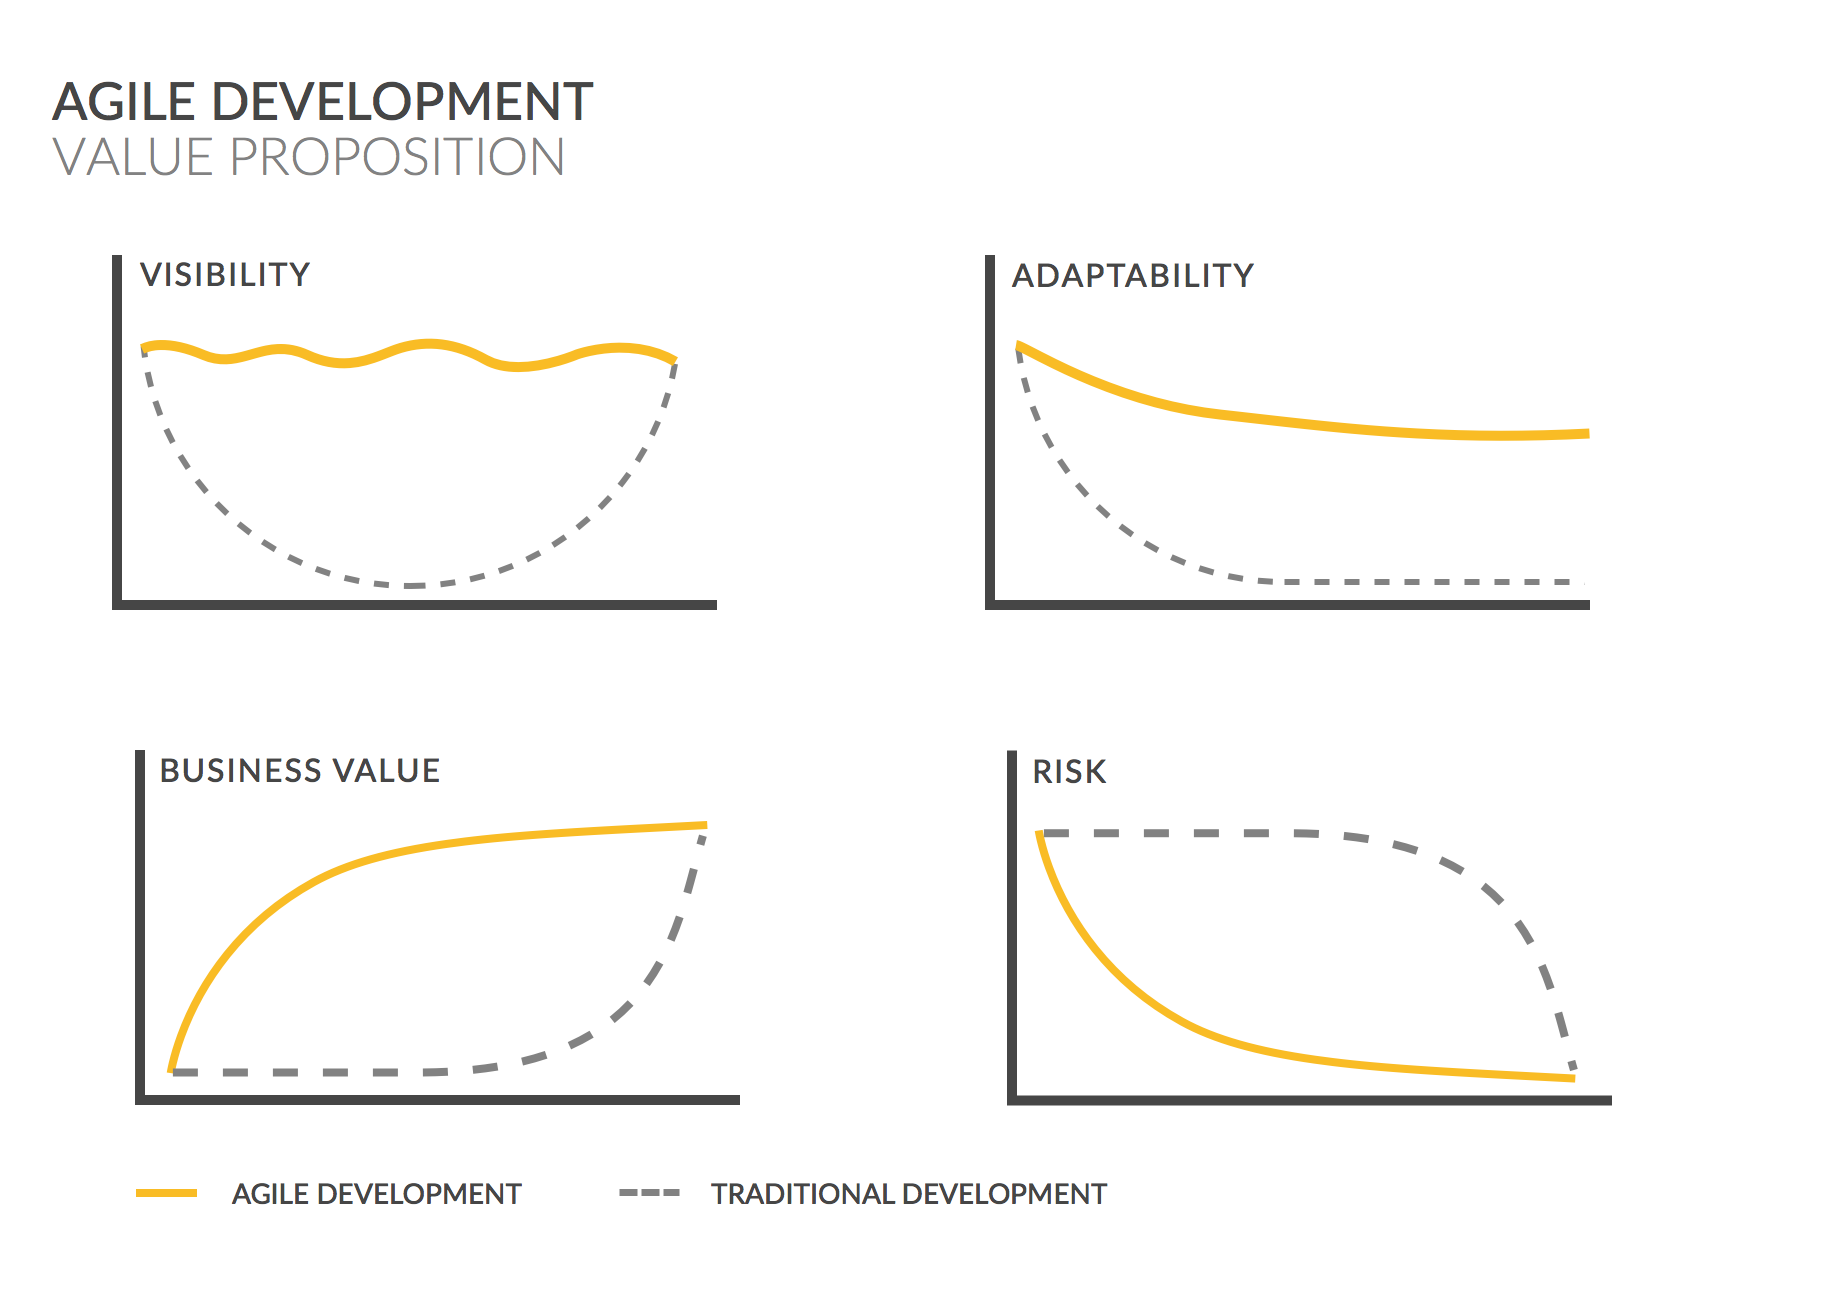
\includegraphics[scale=0.25]{images/travailBP1818/agile.png}
	\centering
	\caption{Comparaison méthodes agiles - traditionnelles}
	\label{agile}
\end{figure}

	Dans notre cas, nous utilisons la méthodologie \textit{Scrum}. Il s'agit de l'une des méthodes agiles les plus utilisée dont nous allons maintenant voir le détail.

\subsection{Déroulement des sprints}

\begin{figure}[h!]
	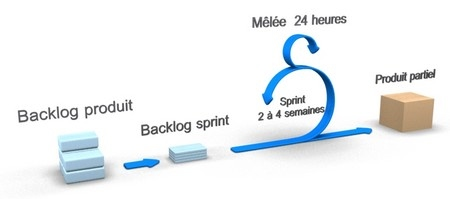
\includegraphics[scale=0.7]{images/travailBP1818/scrum.jpg}
	\centering
	\caption{Méthode Scrum}
	\label{scrum}
\end{figure}

\subsection{Déroulement de la phase de développement}